\section{Introduction} \label{sec:intro}
In the last decades the use of echocardiography is an important clinical approach in Intensive Care Units (ICU) because of the adtages of US devices such as portability, low cost, low radiation and its real-time capabilities to access cardiac anatomy \cite{Feigenbaum1996, Vieillard-Baron2008, singh2007, cambell2018}.
Despite the previous advances, there various challenges in the current practices of clinical ultrasound: 
%are user and patient dependant which can lead to uncertan diagnosis diagnostic.
%\subsection{Challenges in Echochardiography in the ICU}
%\cite{khamis2017} 
%summaries various challenges related to performing echochardiography.

\begin{itemize}
\setlength\itemsep{0em}

\item Intra-view variability of echochardiograms (physiological variations of subjects and adquisition parameters) and sonographer expertise,
 \cite{khamis2017, Feigenbaum1996, field2011}.

\item Inter-view similarity of echochardiograms (similar views of valve motion, wall motion, left ventricle, etc) and transducer position during adquision,
\cite{zhang2018},
redudant information in the clinical echo system (icons, date, frame rate, etc).
\cite{khamis2017}

\item Limited number of expert clinitians to perform US imaging analysis and provice accurate diagnosis, and equipment and hospitalisation requirements in low- and middle-income countries (LMICs)
\cite{hao2021-wellcome}.

\end{itemize}
%Zhang et al. mentioned the challenges of having A4C view with partially osbcured left atrium which might not help to compute left atrial volumes but would help to estimate LV volumes, mass, ejection and longitudinal strain 
%\cite{zhang2018}.
%Particularly, the challenge of locating the right standard views from sonograpehrs of different experiences 
%\cite{Feigenbaum1996}.

%Recent advament of automatic quantificaon if ehcochariography metrics lead to improve such challenges. 
%However, automatic quantification of left ventricular ejection fraction (LVEF) is still challenging at the point of care due to variation of protocols, skills levels \cite{field2011} and the nature of proving feedback on real-time \cite{liu2021}.

%Studies in the management of tetanus in low- and middle-income countries (LMICs) emphasised the importance and requirement of duration of hospitalisation and mechanical ventilation requirements 
%\cite{hao2021-wellcome}.


\subsection{AI-empowered echocardiography}

\cite{hanson2001} reviwed various applications of AI in the ICU where real-time analaysis of waveforms of electrocardiograms and electroencephalograms using neuoral network were used to idenfy cardiac ischemia and diagnosis myocardial ischemia. 
\cite{hanson2001} also reviewed various scnerations where AI is used in the ICU, such as bayesian networks considering central venous pressure (CVP), left ventricular ejection fraction (EF), heart rate (HR), hemoglobin (HGB) and oxygen saturation (O2sat) resulting in a probablitistic cardiac output.
\cite{hanson2001} also touched on datavisualiastion to demonstrate the hypothetical ICU for large number of patients (head injury, sepsis, acute respiratory distress syndrome, etc).

Ghorbani et al. in 2020 reported the first deep learning model to predict age, sex, weight and height from echocardiogram images and make use of such models to understand how models predicts systematic phenotypes which are difficul for human interpreters \cite{Ghorbani-DigitalMedicineNature-JAN2020}.
Authors trained CCN models with 2.6 million echocardiogram images from 2850 patients with the extraction of labels local strucutre and features (e.g. pacemaker lead, dilation of left atrium, hypertrophy for left ventricular) and labels from the physician-interpreted report (e.g, catheters, pacemaker, and defibrillator leads). 
Recently, \cite{hong2022} reviewed 673 papers that made use of machine learning-enabled to help for clinical desicion in the ICU, of these studies the majority used supervised learning (91\%) few doing unsupervising learning and reinforcement learning.
Similarly, \cite{hong2022} identified 20 of the most fequent variables in machine learning-enabled in the ICU, being the top five (age, sex, heart rate, respiratory rate, and pH).
\cite{hong2022} mentioned that typical outcomes in the ICU are mortality, survival, and long-term quality of life and included typical patient outcomes, specific diseases, and stay of time evaluation. 
%For specific diseases, the most studied are sepsis, infection and kidney injury; and trends with liver diseases and severe cancerl and others like cardica diseases, brain diseases;

Tromp et al. classified a dataset of 1145 2D echocardiography videos as apical 4 chamber (A4C) view, apical 2 chamber (A2C) view, parasternal long axis (PLAX) view, or 2D other views and focused versions of the main views \cite{tromp2022}.
Authors used CNN of four layers, dense network and softmax output layer, trained with categorical cross-entropy loss function, then a second classifier of an unsupervised deep learning clustering CNN, trained with mean square error and Kullback-Leibler loss functions \cite{tromp2022}.
%For the remaining dataset (2,126 PSAX-PM echo cines), while the LV segmentation is not available, the ground truth LVEF values are acquired from the patients’ archived information.

\cite{zhang2022-mdpi}
reviewed AI's applications in left ventricular systolic funciton (LVEF) and global longitudinal strain (GLS), pointing out its dependendant to the sonographers's expertise (inter-observer variability) and post-processing and variablity in differen US devices.
\cite{zhang2022-mdpi} pointed the challenges of AI-enhanceed echocargiografy for interpretability of results and its sensitivity to sample shortage, to which authors mention about the potentials of multimodal imaging (us, mri and clinical data) to improve detection rate of diseases. 

\cite{behnami2020} applied DenseNet-like network for feature learning and RNN unit with bidirectional Gated Recurrent Units to alivate loss of information from the ealier frames of echos to automatically detect high risk or low risk of heart failure with reduced ejection fraction with an overall accuracy of 83.15\%, precision of 82.6\% and recall of 81.1\%.
\cite{behnami2020} mentioned that EF is highly user-dependant to which they propose to collect more data,

\cite{liu2021JMIA} proposed pyramid local attention neural network (PLANet) to improve segmentation performance of automatic methods in 2D echocardiography.
PLANet was evaluated with CAMUS and sub-EchoNet-Dynamic datasets, showing a better performance against geometric and clinical metrics.

\cite{ulloaCerna2021} made use of DNN to learn spatiotemporal features from echocardiography video data to enhance clinical prediction of 1 yr all-cause mortality where video echo data linked to EHR data that included hand-crafted echocardiography-derived measurements (EDMs), additional clinical variables and individual outcomes.
The DNN model presents "superior prediction performance" over four cardiologist and two benchmark clinical models: the pooled cohort equations (PCE) and Seattle Heart Failure (SHF) risk score \cite{ulloaCerna2021}. 
\cite{ulloaCerna2021} used "full, raw (annotation-free) echocardiographic videos to make predictions by learning from more than 812,278 clinically acquired echocardiography videos of the heart (50 million images)."

\cite{jafari2021} pointed out the challenges of obtained high quality for less experience operators and the hight variablity or echo quality adn cardiovascular structures accross different patients to which authors proposed "Bayesian deep learning approach for fully automatic LVEF estimation based on segmentation of the left ventricle (LV) in parasternal short-axis papillary muscles (PSAX-PM) level". 
\cite{jafari2021} made use of 2,680 patients with PSAX-PM echo cine acquired by a variety of ultrasound devices, namely iE33, Vivid i/7/9/95, Sonosite, and Sequoia (only 554 echo cines were considered as ground truth with LV mask delineated by an experienced level III
echocardiographer).

Ono et al. applied differen models where Unet++ demonstrated good performance for automatic endocardial border detection and left ventrical assesment in 2D echocardiographu videos \cite{ono2022}.
The datasets to train networks was made of 2798 images from 118 videos of which 22 videos with 465 frames were for 4CV \cite{ono2022}.
Ono et al. also touched on the challenges of providing explainable AI for US imaging.

\subsection{Real-time AI-empowwered echocardiography}
In terms of real-time analysys of echocardigraphy, , Wu et al. 2022 applied baselines of UNET with temporal context-aware encoder (TCE) and bidirectional spatiotemporal semantics fusion (BSSF) modules to EchoDynamic (10030 video sequences with of 200frames of 112x112 pixes) and CAMUS datasets  (450 video of 20 frames of 778x594 pixels) with evaluation metrics of Dice score (DS), Hausdorff Distance (HD), and area under the curve (AUC) \cite{wu20222}.
Wu et al. 2022, ensuring low latency and real-time performance, presented speed analysis againts eight methods using calculations number FLOPS (G), number of parameters (M) and speed ($ms/f$) which lowest one was 32 $ms/f$  \cite{wu20222}.

\begin{table}[]
\tiny
\begin{tabular}{llllllll}
\textbf{Author(s), year} & \textbf{Datasets (clips)}           & \textbf{Input}        & \textbf{Flops} & \textbf{Model;} & \textbf{Latency}  & \textbf{Hyper-}      & \textbf{Code} \\
                         &                                     & \textbf{frames}       &                & \textbf{Params}      &                   & \textbf{parameters}  &               \\
\cite{wu20222}           &  EchoDynamic (10Kc)                 & 3                     & 56.359         & TCE-BSSF;74.798      & 32 (ms/f)         & lr=10e-4;epochs=100; & -             \\
                         &  CAMUS (.5Kc)                       &                       &                &                       &                   & CR=5-fold            &          \\
\cite{woudenberg2018}    & AP4(2Kc)                            & 10                    & -              & DenseNet-LSTM;        & 352.91ms          & -                    & -             \\
                         &                                     &                       &                &                       &                   &                      & - \\
\cite{ostvik2021-TMI}   & Synthetic/Simulated/Clinical         & 7                     & -              & Echo-PWC-Net          & -                   & -                      & -
\end{tabular}
\end{table}
%by https://www.tablesgenerator.com/


%EchoDynamic (10030 clips with of 200frames of 112x112 pixes)
%CAMUS (450 clips of 20 frames of 778x594 pixels)
%TCE: temporal context-aware encoder. BSSF: bi-directional spatiotemporal semantics fusion

%TODO
%* Read relevant work of sophie yacoub and C Louise Thwaites that can be related to our work!
    %https://scholar.google.com/citations?user=gjZ_bDkAAAAJ
    %https://scholar.google.com/citations?user=YLCVWQoAAAAJ



\section{Methods for AI-empowered echocardiopgraphy}

\subsection{Image Quality Assessment}
\cite{labs2021_in_miua} considers chamber clarity, depth gain, on-axis attributes, apical foreshoredness.

\subsection{Classification of echochardiograms}
\cite{woudenberg2018} applied DenseNet and LSTM to extract temporal information on sequences of 16K echo cine frames to classify 14 heart views with an average accuracy of 92.35\%.
\cite{woudenberg2018} implemented a Tensorflow runner that performs contrast enhancement to then sent each frame to three identical CNNs running in separated threads to prevent lag during inference times.
Then a shared buffer collects extracted features from CNNs to then awake the thread for the LSTM network from the previous ten frames to produce classification and quality prediction.
\cite{woudenberg2018} also presents timing diagrams to quantify frame arrival and real-time performance to operate at 30 frames per second, while providing feedback with a mean latency of 352.91 ± 38.27 ms when measured from the middle of the ten-frame sequence.

Zhang et al. performed view classification with 277 echochardiograms to create a 23-class models (including a4c no occlusions, a4c ocluded LA, a4c ocluded LV, etc) using 13-layer CNN with 5-fold cross-validation for accuracy assement and resulting in 84\% for overall accuracy where challenges for partial obscured LVs for a2c, a3c and a4c \cite{zhang2018}.
Similarly, Zhang et al. applied U-net to segment 5 views (a2c, a3c, a4c, PSAX, PLAX) and CNN model for 3 chardiac disseases with the use of A4c captuting most of the information for the diseases.

Khamis et al. considered 309 clinical echocardiogram of apical viewss which were visiually classified and labelled by two experts into three classes: 103 a2c views, 103 a4c views and 103 alx views to then applied spatio-temporal feature extraction (Cuboic Detector) and supervised learning dictionary (LC-KSVD) resulting in an overall recognition rate of 95\% \cite{khamis2017}.

\subsection{Clustering techniques}
Zhang et al. mentioned that 23 view classes from 7168 individually labeled videos that ware classified with a 13-layer CNN to then viewed with the use of t-Distributed Stochastic Neighbor Embedding \cite{zhang2018}.
Zhang et al. made use of 277 echochardiograms collected over a 10-year period for view classification.
Kusunose et al. mentioned that other authors have reached an acciracy of 91-94 for 15-view classification while their work mentioned a 98.1 accuracy for five-prederminted views \cite{kusunose2021}.

\subsection{Auto-encoders}
Laumer et al. proposed a novel autoencoder-based framework to learn human interpretable representation of cardiac cycles from cardiac ultrasound data \cite{laumer2020},
%Further reading:
%https://arxiv.org/pdf/2112.02102.pdf
%https://ieeexplore.ieee.org/abstract/document/8051114

Ouyang et al. presented echo-dynamic dataset as the first annotated medical video dataset with 10,036 videos. 
Additionally, authors reported the use of three CNN arquitectures varing filters in each layer to assess ejection fraction to near-expert performance.
It is worthwhile to note that authors got best performance with mean absolute error of 5.44\% using clip lenght of 16 and frame rate of 4.
Such error is near-expert perfonace as they can get 4-5\% for skilled echochardiographers in cotrolled settings \cite{ouyang-NeuripsML4H2019}.


Ghorbani et al. applied convolutional neural networks of cardiac ultrasound to identify local structures, estimate cardiac function and predict pathologies.
Their deep learning model, EchoNet, can identify up to 10 cardiac biometrics which results in decreasing repetitive task in the clinical flow, provide interpretation to less experienced cardiologist, and predict phenotipes. This work can predict age, sex, weight and heigth from echocardiogram images. 
Authors mention that the increase of date does not improve model traiining. The homogenisation of cadiac views prior to model training improved training speed and computaitonla time \cite{Ghorbani-DigitalMedicineNature-JAN2020}


\subsection{Segmentation}
With the challenges of limited sampling of cardiac cycles and the considerable inter-observer variability, Ouyang et al. presented a CNN model with residual connections and spatiotemporal convolutions that surpase human performance of segmentaion of left ventricle, estimation of ejection fraction and assessment of cardiomyophaty. 
Their model reached Dice similarity coefficient of 0.92, predicts ejection fraction with mean absolute error of 4.1\% and clasify heart failure based on reduced ejection fraction 
%Wonder is relevant to predic and classify with our datasets in the ICU?  Fri  7 Jan 14:42:23 GMT 2022
\cite{Ouyang-Nature-APR2020}.


Meyer et al. used Prominence Iterative Dijkstra’s algorithm (ProID), based on the identification of ventricle boundaries with iterative Dijkstra's algorithm, for ventricle detection and volumen estimation \cite{Meyers2020}.
ProID employs echochardiogram-specific cost-matrix to address contrast-to-noise and resolution limitations problems \cite{brindise2020unsupervised}.


\subsection{Contrastive Learning}
Methods on Contrastive Learning apparently address the challenge of required labelled data to identify pathologies in the images of dectect certain cardiac views.
Recently, Chartsias et al. use contrastive learning to train imbalanced cardiac datasets and they compared a naive baseline model to achieve a F1 score of up to 26\% \cite{chartsias2021-ASMUS}
Saeed et al. recently investigated contrastive pretraining to improve the DeepLabV3 and UNET segmentation networks of cardiac structers in ultrasound imaging.
Authors showed comparable results with state-of-the-art fully supervised algorithms and presents better results compared to EchoNet-Dynamic and CAMUS \cite{saeed2021MIDL}





\subsection{AI-guided US imaging}

Near-human quantification of LV and EF has been investated, however Asch et al. pointed out that buoundary identification is prone to errors when low quality images or artifacts are used
Asch et al. pointed out that data and materials were not publicly available and they made use of AutoEF by captionhealth co.
Authors used a databes of 50000 echocardiography datasets over a period of 10 years of varios clinical US syustems. 
The training datasets included multiople views of 2 and 4-chamber views and LV EF values where clininias use conventional methods (biplane Simpson technique) \cite{asch2019CIRIMAGING}.

Asch et al. \cite{asch2021CircImaging}.

Hong et al. reported the evalition of imagin quality asssement to demostrated that AI can recognise nuaces of varing imaing during scanning \cite{hong2021JACC}


Narang et al. reported the adquisiton of 10 echocardiography views of novices users using deep-learning-based software \cite{Narang2021JAMACARDIOLOGY}.
Narang et al. mentioned that CNN were used with stacks of networks and transofrmations. 
The AI-guided software consist of three estimates: (1) quality image assement, (2) "6-dimensional geometric distance with postion and orientation between the current probe location and the locattion anticipated to optimise the image"; and (3) corrective probe manipulation. \cite{Narang2021JAMACARDIOLOGY}
Authors mention that algorithms do not use trackers, fiducial marks or additional sensors to made guide estimations \cite{Narang2021JAMACARDIOLOGY}.


Cheema et al. reported the use of AI-enabled guidance to sonoographer which was created from the use of 500000 hand movmentes.
Cheema et al.  reported that such feature was the first cardiac aotorhisedd by Food and Drug adminstation in 2020. 
Authors presented five cases covid-19 intensive care unit (ICU) to illustrate "how desition making affect in patient care" and how the use of AI-enabled provided real-time guidance to acquire desired cardiac UL with the sterting of user's transducer position and hand movevemnt \cite{CHEEMA2021JACCCaseReports}.



\subsection{3D US}
Considering that 3D left ventricle (LV) can provide full volume information of the hearth than 2D echordaiography,  Dong et al. proposed a real-time framework VoxelAtlasGAN that made use of cGAN \cite{dong2018-MICCAI}. 
VoxelAtlasGAN framework with mean surface distance of 1.85 mm, mean hausdorff distance of 7.66mm, mean dice 0.953 and correlation of EF 0.918 and the mean inference speed of 0.1 s demostrated potential for clinical applicaiton \cite{dong2018-MICCAI}.
Dong et al. in 2020 applied tranformers to obtain translations parematers that passed to VoxelAtlasGAN \cite{dong2020-MIA}.
AlasNET framework  ended up with "mean surface distance, mean hausdorff surface distance, and mean dice index were 1.52 mm, 5.6 mm and 0.97 respectively" \cite{dong2020-MIA}

Smistad et al. 2021 made use of CETUS 3D US LV segmentation dataset and weakly annorated datasets for real-time 3D left ventricle segmentation and estiomation of ejection fraction \cite{smistad2021-D-IUS}.
Authors presented the impact of pre-training that resulted in an improvement of Dice score. 
It is imporant to note that VoxelAlasGAN and AtlasNet by Dong el al. presented a better dice score.
Smistad et al. 2021 concluded that a limited labelled datasets of 15 patiens demostrate good accuracy and models were able to generalise to new data and ultrasoudn scanners \cite{smistad2021-D-IUS}.




\subsection{Transformers}

Rubin et al. noted the shortcoming of transformers of extensive compation for training that lead to use detection transformer (DETR) which make smaller models reducing model size and acceleration inference \cite{rubin2021-PMLH}.,
Rubin et al. considered the detection of needles in real-time ultrasound video sequences 12,000 needle insertions (2 million of individual frames).
Video sequences (up to 60 sec in time) were divided into 30-frame clips (1 sec in time).


Reynaud et al. 2021 adapted Residual Autoencoder Network and BERT model to predict ejection fraction which is different from what is commonly use with segmentation methods \cite{reynaud2021-MICCAI}.
Reynaud et al. applied their model to Echonet-Dynamic dataset which only constains 10,030 echocardiograms containing one to three or more cadiac cycles with only cardiac cycle with ES and ED annorations.
Due to the distribution between ES and ED, the sequence legnth was 128 frames.
As Echonet-Dynamic datasets contains unlabelled ES and ED, Reynaud et al. applied (a) Guided Random Sampling (b) Mirroring Methods.
Code is available at \url{https://github.com/HReynaud/UVT}.



\subsection{Others}
Rank-2 non-negative matrix factorization \cite{yuan2017} to generate End-Systole and End-Diastole for apical 4 view.  
Recently Robust Non-negative Matrix Factorization seems to be implement low-computation cost algorithms to automatic segment mitral valve \cite{dukler2018}.

Salte et al. classified three standard appical views from data of 200 patients to peformf straing measurements with deep learning arquitectures \cite{SALTE2021-JACC}.
Salte el al. made use of the work \cite{ostvik2021-TMI} inception and dense network were used to clasity, recurrent network to detect event timing and u-net-based network for segmentation \cite{SALTE2021-JACC}.
Authors compared the results with the commenrially avaible semiautomatic speckle-tracking software (EchoPAC v202), reporting evinde of the comparable GLS measurmentes to other semiatuomatic methods \cite{SALTE2021-JACC}.




\section{Spatiotemporal Features}


\subsection{Deep Residual Learning}
Ouyang et. al. benmarked various spatiotemporal convolutions (Sports-1M, Kinetics, UCF101, and HMDB51) \cite{ouyang-NeuripsML4H2019}  based on deep residual learning (He et al. 2015 and Tran et al. 2018).

%"In the interest of creating high performance baselines on standard videos with gray-scale images without
%proprocessing or creation of optical flow frames, we evaluated the performance of three architectures
%which combine 3D convolutions over spatiotemporal video volume with residual connections between
%layers[32]. Each model uses ResNet-18 as the base architecture and consists of 18 convolutional
%layers with residual connections connecting odd numbered layers [16].

%32:  
%A Closer Look at Spatiotemporal Convolutions for Action Recognition
%single type of network (ResNet) and a homogenous use of our (2+1)D spatiotemporal decomposition
%https://openaccess.thecvf.com/content_cvpr_2016/html/He_Deep_Residual_Learning_CVPR_2016_paper.html32: 
%https://arxiv.org/pdf/1711.11248.pdf

%16:
%Deep Residual Learning for Image Recognition 
%He et al. 2015
%https://arxiv.org/abs/1512.03385


\subsection{LSTM}
Recently, Smistad et al. 2021 presented the use of LSTM to address the single frame segmentation of end-diastole and end-systole to address segmentation fricklering and reduce tmeporal errors \cite{smistad2021-C-IUS}.
One of the challenges is architecture design to add ConvLSTMs to whcih authors experiment at the location at the endocer, decoder, last layer and in bottlenet, to which authors mentiosn that the use of the ConvLSTM layers in the encoder of the temporal NN gave the best results \cite{smistad2021-C-IUS}.
Authors mention that interpolation of the annorations of the entire cardiac cycle did not captured the complex motion witht he use of 7 frames to which they suggest to use advance speckle tracking such as Echo-PWC-Net  \cite{ostvik2021-TMI}.

Lu et al. made use of U-Net and LSTM to model Left Ventricular cardiac motion \cite{lu2020-MIUA}.

Bar et al. assessed surgical workflow recongnition and report a deep learning system in wich clips of one second to create a short-term spatio-temportal model based on inflated 3D network with non-local to optain SoftMax probability vector to fed LSTM to produce final phase predictions \cite{Bar2020}

\section{Validation and Usability Studies}
Francesconi et al. 2021 presented technical vaidation by intra-operator reproducbility of two measuremnts (intima-media thickness and distension) by one expert and usability of integrated system in a laboratory setting with 12 healthy volunteers \cite{francesconi2021}.

\section{Cardiac Motion Estimation}
Cardiac motion estimation has important role in echocardiography due to the computation of myocardial deformation indices. 
\cite{aviles2017} propose a method to estimate cardiac motion of ultrafast ultrasound data by combining low-rank data representation with topology preservation to
overcome the challenges of non-rigid registration that involves complex heart motion and distortions.
\cite{ahn2022} proposed a method to build 3D recovery models from 2D echocardiography data with the only assumption that the probe is fixed for one cardiac cycle.
\cite{evain2022-medimag-ieee} proposed a deep learning model PWC-Net, achieving an average endpoint error of 
"0.07± 0.06 mm per frame and 1.20±0.67 mm between ED and ES on their simulated dataset".
See \cite{ostvik2021-TMI} for further details on Echo-PWC-Net and other networks. 

\section{Datasets in echocardiography}

%\subsection{}
%* Alberta Heart Failure Etiology and Analysis Research Team; HEART; n=1029 echocardiograms), a
%* real-world dataset from Taiwan (n=31 241)
%\cite{tromp2022}.

\subsection{CAMUS (2D US)}
CAMUS dataset, Cardiac Acquisitions for Multi-structure Ultrasound Segmentation, was publised in 2019 by Leclerc et al. 2019 \cite{leclerc2019-IEEETransMedicalImaging}.
CAMUS is the largest publicy-available and fully-annotated dataset of two and four-chamber adquistion from 500 patients.
Datasets is cathegorised in image quality (good, medium, and poor) and $LV_{EF}$ ($\leq$ 45\% (phatological risk) , $\geq$ 55\%, else).
The dataset reflects a daily clinical practice data where images quality and a range of phatological cases.
Dataset was collected with GE Vivid E95 ultrasound scanners (GE Vingmed Ultrasound, Horten Norway) with a GE M5S probe (GE Healthcare, US).
The datasets is available electronically to download at \url{https://www.creatis.insa-lyon.fr/Challenge/camus/}.
%Non-deep-learning techniques analyse cardiac cycles to analysis end-diastole and end-systolic left ventricular volumes with a mean correlation of 0.95 and absolute mean error of 9.5 ml.

\subsection{EchoNet-Dynamic (2D US)}
Ouyang et al. published a large datasets of 10,030 annotated echocardiogram videos \cite{ouyang-NeuripsML4H2019, Ouyang-Nature-APR2020}.
Datasets were labelled left ventricle volumes by sonographers to calculate ejection fraction.
Datasets were acquired by skilled sonographers using iE33, Sonos, Acuson SC2000, Epiq 5G or Epiq 7C ultrasound machines and processed images were stored in a Philips Xcelera system.
The datasets is available electronically to download at \url{https://echonet.github.io/dynamic/index.html#dataset}.
%he resulting square images wereeither 600 × 600 or 768 × 768 pixels depending on the ultrasoundmachine and down sampled by cubic interpolation using OpenCVinto standardized 112 × 112 pixel videos.

\subsection{CETUS (3D US)}
Challenge on Endocardial Three-dimensional Ultrasound Segmentation (CETUS) dataset was published in 2016 by Bernard et al. \cite{bernard2016TMI}.
CETUS contains 45 sequences of 3D ultrasound volumes of one cardiac cycle from 45 patients were equally acquired from three different hospitals with three different brands of ultrasound machines (GE, Philips and Siemens) \cite{bernard2016TMI}.
The studied population of 45 participants is composed of 15 healthy subjects, 15 with previous myocardial infartation, 15 with dilated cardiography.
The datasets is available electronically to download at \url{https://www.creatis.insa-lyon.fr/EvaluationPlatform/CETUS/about_database.html}.

\subsection{Synthetic cardiac motion}
Alessandrini et al. in 2018 published "a open access library of 105 synthetic sequences encompassing i) healthy and ischemic motion patterns, ii) most common apical probe orientations iii) vendor specific image quality from 7 different systems" \cite{alessandrini2018}.
See previuos work of Alessandrini et al. in 2015  \cite{alessandrini2015_isbi}.
%TOCHECK: https://ieeexplore.ieee.org/abstract/document/9594689

\section{Tools}

\subsection{Annotation tools}
Recently, Smistad et al. 2021 published the first web-based tool for annoration of medical ultrasound video to do image classification, segmentation, bouding box and landmark annotation  \cite{smistad2021-A-IUS}.
AW tool has been used since 2016 at different projects to perform segmentation of the left ventricle, cardiac view classification, and detection of nerves and blood vesels \cite{smistad2021-A-IUS}.

\section{Methods and materials}

\subsection{Proposed model}
\begin{figure}[h]
\centerline{
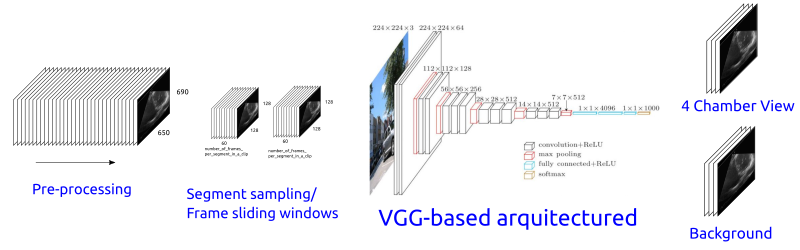
\includegraphics[width=\columnwidth]{../figures/VGG-based-arquitecture/versions/drawing-v00}
}
\caption{
	VGG-based arquitecture
	(\textbf{a}) description...
	(\textbf{b}) description...
	Figure is adapted from the works of %\cite{}.
}
\end{figure}



\section{Datasets}

\subsection{VITAL}
86 patients of average age (?) ? male and ? female were collected by four clinicians of ? years of expience collected echochardiography datasets.
The collection was done with the clinical device GE Venue Go machine and GE convex probe C1-5-D.

\begin{figure}[h]
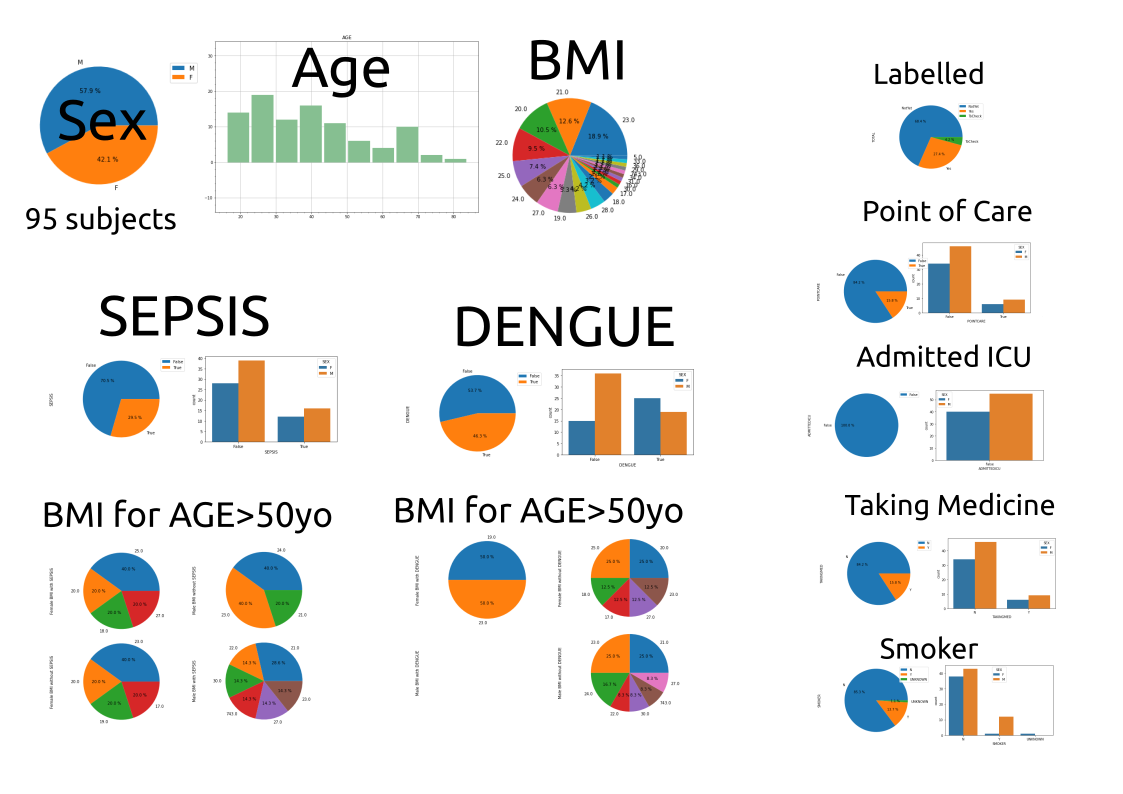
\includegraphics[width=\columnwidth]{../figures/patient-demographics-and-diseases/versions/drawing-v00}
\caption{
	Patient demographics
	(\textbf{a}) description...
	(\textbf{b}) description...
	Figure is adapted from the works of %\cite{}.
}
\end{figure}


\subsection{Ethics statement}
This study was approved by ... and the ethics committee ...
All participants gave written informed consent to participate before enrollment.

\section{Potential future work}
2D velocity vector fields of flow blow can help to detect abnormal flow patterns as done in fetal and neonatal echochardiograhy \cite{Meyers2020}.
Use LV A4C echos that can create synthetic Ulstraound images for GE Vivid E9, Hitachi Prosound U7, Philips iE 33 Vision, Siemens SC2000, and Toshiba Artida ultrasound systems \cite{brindise2020unsupervised}. 
